%!TEX program = xelatex
\documentclass[11pt]{beamer}

\usepackage{amsfonts}
\usepackage{amsmath}
\usepackage{blindtext}
\usepackage{enumitem}
\usepackage{fancyvrb}
\usepackage{tikz}

\usetheme{SaoPaulo}

\title{Numerical Python}
\subtitle{numpy.array, plotting}
\author{CS101 Lecture \#15}
\date{2016-11-14}

\setcounter{showSlideNumbers}{1}

\newcommand{\correctstar}{\textcolor{red}{$\star$}}

\begin{document}
  \setcounter{showProgressBar}{0}
  \setcounter{showSlideNumbers}{0}

%%%%%%%%%%%%%%%%%%%%%%%%%%%%%%%%%%%%%%%%%%%%%%%%%%%%%%%%%%%%%%%%%%%%%%%%%%%%%%%%
\frame{\titlepage}

%%%%%%%%%%%%%%%%%%%%%%%%%%%%%%%%%%%%%%%%%%%%%%%%%%%%%%%%%%%%%%%%%%%%%%%%%%%%%%%%
\setcounter{framenumber}{0}
\setcounter{showProgressBar}{1}
\setcounter{showSlideNumbers}{1}


%%%%%%%%%%%%%%%%%%%%%%%%%%%%%%%%%%%%%%%%%%%%%%%%%%%%%%%%%%%%%%%%%%%%%%%%%%%%%%%%
\section{Warm-up Questions}


%%%%%%%%%%%%%%%%%%%%%%%%%%%%%%%%%%%%%%%%%%%%%%%%%%%%%%%%%%%%%%%%%%%%%%%%%%%%%%%%
\begin{frame}[fragile]
  \frametitle{Multidimensional indexing}
  \Enlarge
  
a = [ [1, 2], [3, 4], [5, 6, 7] ]

\begin{enumerate}
\myitem What is the type of \texttt{a}?
\myitem What is the value of a[2][2]?
\myitem What is the value of a[1][2]?
\end{enumerate}

\end{frame}


%%%%%%%%%%%%%%%%%%%%%%%%%%%%%%%%%%%%%%%%%%%%%%%%%%%%%%%%%%%%%%%%%%%%%%%%%%%%%%%%
\begin{frame}[fragile]
  \frametitle{Multidimensional indexing}
  \Enlarge
Create the following two-dimensional list:
  
\begin{Verbatim}
x = [ [1,0,0,0],
      [0,1,0,0],
      [0,0,1,0],
      [0,0,0,1] ]
\end{Verbatim}


\end{frame}

%%%%%%%%%%%%%%%%%%%%%%%%%%%%%%%%%%%%%%%%%%%%%%%%%%%%%%%%%%%%%%%%%%%%%%%%%%%%%%%%
\section{Array}

%%%%%%%%%%%%%%%%%%%%%%%%%%%%%%%%%%%%%%%%%%%%%%%%%%%%%%%%%%%%%%%%%%%%%%%%%%%%%%%%
\begin{frame}[fragile]
  \frametitle{The problem}
  \Enlarge

  \begin{Verbatim}
mydata = [ 4.5, 6.0, 1.2, 5.4 ]
from math import sin
sin(mydata)
  \end{Verbatim}
  %\pause
  \begin{enumerate}
  \myitem  Why doesn't this work? %\pause
  \mysubitem  \texttt{list} can contain any type!
  \myitem  Also operators don't do what we ``want":
  \end{enumerate}
  \begin{Verbatim}
mydata * 2.0  # doesn't double values!
  \end{Verbatim}
\end{frame}

%%%%%%%%%%%%%%%%%%%%%%%%%%%%%%%%%%%%%%%%%%%%%%%%%%%%%%%%%%%%%%%%%%%%%%%%%%%%%%%%
\begin{frame}[fragile]
  \frametitle{\texttt{numpy.array}}
  \Enlarge

  \begin{Verbatim}
import numpy
import numpy as np  # better way
  \end{Verbatim}
  %\pause
  \begin{enumerate}
  \myitem  \texttt{numpy} provides arrays and mathematical functions.
  \end{enumerate}
  \begin{Verbatim}
data = np.array( [ 4.5, 6.0, 1.2, 5.4 ] )
data * 2.0
np.exp(data)
  \end{Verbatim}
\end{frame}


%%%%%%%%%%%%%%%%%%%%%%%%%%%%%%%%%%%%%%%%%%%%%%%%%%%%%%%%%%%%%%%%%%%%%%%%%%%%%%%%
%%%%%%%%%%%%%%%%%%%%%%%%%%%%%%%%%%%%%%%%%%%%%%%%%%%%%%%%%%%%%%%%%%%%%%%%%%%%%%%%
%\section{More \texttt{numpy}}

%%%%%%%%%%%%%%%%%%%%%%%%%%%%%%%%%%%%%%%%%%%%%%%%%%%%%%%%%%%%%%%%%%%%%%%%%%%%%%%%
\begin{frame}[fragile]
  \frametitle{Indexing arrays}
  \Enlarge

  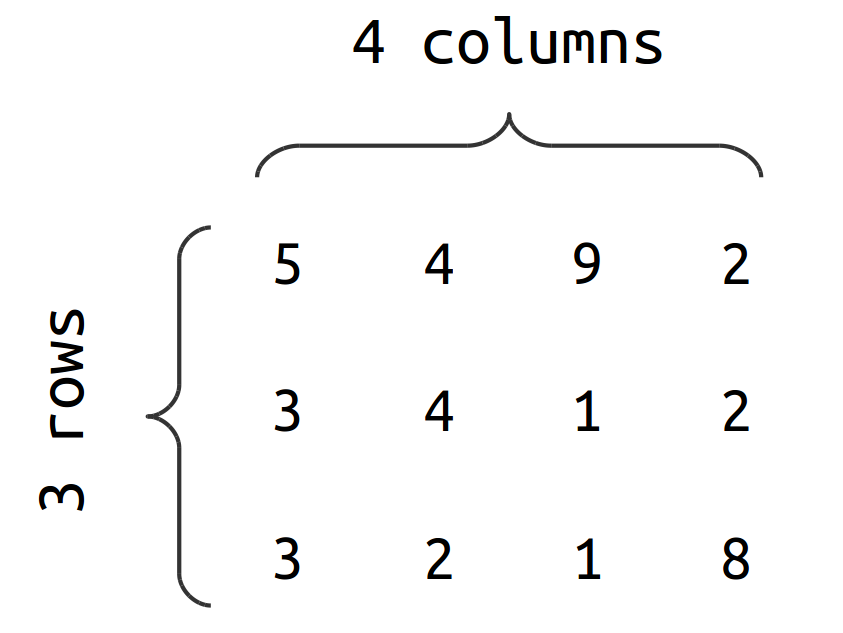
\includegraphics[width=0.67\textwidth]{./img/ndarray.png}

  \begin{enumerate}
  \myitem  \texttt{numpy.array} indexes an element by \texttt{array[row][col]}.
  \myitem  \texttt{numpy.array} indexes a row by \texttt{array[row]}.
  \myitem  \texttt{numpy.array} indexes a sub-array by \texttt{array[r1:r2, c1:c2]}.
  \end{enumerate}
\end{frame}

%%%%%%%%%%%%%%%%%%%%%%%%%%%%%%%%%%%%%%%%%%%%%%%%%%%%%%%%%%%%%%%%%%%%%%%%%%%%%%%%
\begin{frame}[fragile]
  \frametitle{Indexing arrays}
  \Enlarge

  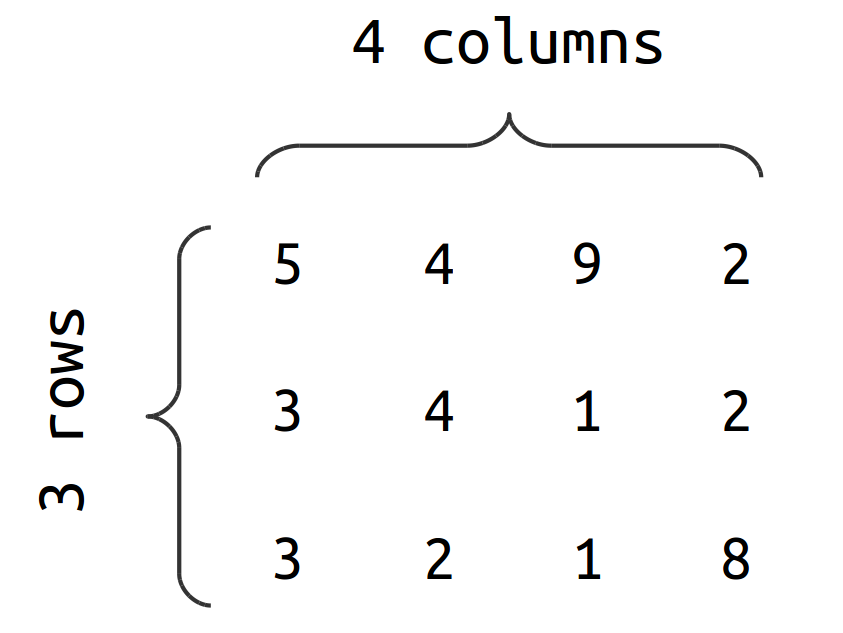
\includegraphics[width=0.67\textwidth]{./img/ndarray.png}

  \begin{enumerate}
  \myitem  What is \texttt{a[1:3][1:2]}?.
  \end{enumerate}
\end{frame}

%%%%%%%%%%%%%%%%%%%%%%%%%%%%%%%%%%%%%%%%%%%%%%%%%%%%%%%%%%%%%%%%%%%%%%%%%%%%%%%%
\begin{frame}[fragile]
  \frametitle{Question}
  \Enlarge

$$
x =
\left(
\begin{array}{cc}
1 & 1 \\
2 & 2 \\
3 & 3
\end{array}
\right)
$$

  What will produce this array?

  \begin{enumerate}[label=\Alph*]
  \item
  \begin{Verbatim}
np.array([[1,2,3],[1,2,3]])
  \end{Verbatim}
  \item
  \begin{Verbatim}
np.array([2,3])
  \end{Verbatim}
  \item
  \begin{Verbatim}
np.array([3,2])
  \end{Verbatim}
  \item
  \begin{Verbatim}
np.array([[1,1],[2,2],[3,3]])
  \end{Verbatim}
  \end{enumerate}
\end{frame}

%%%%%%%%%%%%%%%%%%%%%%%%%%%%%%%%%%%%%%%%%%%%%%%%%%%%%%%%%%%%%%%%%%%%%%%%%%%%%%%%
\begin{frame}[fragile]
  \frametitle{Question}
  \Enlarge

$$
x =
\left(
\begin{array}{cc}
1 & 1 \\
2 & 2 \\
3 & 3
\end{array}
\right)
$$

  What will produce this array?

  \begin{enumerate}[label=\Alph*]
  \item
  \begin{Verbatim}
np.array([[1,2,3],[1,2,3]])
  \end{Verbatim}
  \item
  \begin{Verbatim}
np.array([2,3])
  \end{Verbatim}
  \item
  \begin{Verbatim}
np.array([3,2])
  \end{Verbatim}
  \item
  \begin{Verbatim}
np.array([[1,1],[2,2],[3,3]])
  \end{Verbatim}
  \correctstar
  \end{enumerate}
\end{frame}


%%%%%%%%%%%%%%%%%%%%%%%%%%%%%%%%%%%%%%%%%%%%%%%%%%%%%%%%%%%%%%%%%%%%%%%%%%%%%%%%
\begin{frame}[fragile]
  \frametitle{\texttt{numpy.array}}
  \Enlarge

  Consider a data set containing patient inflammation records for 60 patients over a period of 40 days, contained in \texttt{inflammation.csv}.

  \begin{Verbatim}
data = np.loadtxt( './data/inflammation.csv',
                   delimiter=',' )
  \end{Verbatim}
\end{frame}

%%%%%%%%%%%%%%%%%%%%%%%%%%%%%%%%%%%%%%%%%%%%%%%%%%%%%%%%%%%%%%%%%%%%%%%%%%%%%%%%
\begin{frame}[fragile]
  \frametitle{\texttt{numpy.array}}
  \Enlarge

  \includegraphics[width=\textwidth]{./img/axes.png}
\end{frame}


%%%%%%%%%%%%%%%%%%%%%%%%%%%%%%%%%%%%%%%%%%%%%%%%%%%%%%%%%%%%%%%%%%%%%%%%%%%%%%%%
\begin{frame}[fragile]
  \frametitle{\texttt{numpy} Data types}
  \Enlarge

  \begin{enumerate}
  \myitem  \texttt{numpy} supports many possible data types:
    \begin{enumerate}
    \mysubitem  \texttt{bool}
    \mysubitem  \texttt{int16}, \texttt{int32}
    \mysubitem  \texttt{float16}, \texttt{float32}, \texttt{float64}
    \mysubitem  \texttt{complex64}, \texttt{complex128}
    \end{enumerate} %\pause
  \myitem  For the most part, stick with \texttt{bool}, \texttt{int32}, and \texttt{float64} (most accurate).
  \myitem  Specify (and query) with \texttt{dtype}:
  \end{enumerate}
  \begin{Verbatim}
import numpy as np
a = [ 3,2,4 ]
x = np.array( a,dtype=np.float64 )
x.dtype
  \end{Verbatim}
\end{frame}



%%%%%%%%%%%%%%%%%%%%%%%%%%%%%%%%%%%%%%%%%%%%%%%%%%%%%%%%%%%%%%%%%%%%%%%%%%%%%%%%
\begin{frame}[fragile]
  \frametitle{Other arrays}
  \Enlarge
  \begin{Verbatim}
x = np.zeros([2,3] ) # zeroes
y = np.ones([4,1])   # ones, 4 rows, 1 column
y = np.ones([1,4])   # ones, 1 row, 4 columns
y = np.ones([4])     # ones, a row vector
  \end{Verbatim}

  \begin{enumerate}
  \myitem  Produce arrays of zeros or ones with specified dimensions.
  \end{enumerate}
\end{frame}

%%%%%%%%%%%%%%%%%%%%%%%%%%%%%%%%%%%%%%%%%%%%%%%%%%%%%%%%%%%%%%%%%%%%%%%%%%%%%%%%
\begin{frame}[fragile]
  \frametitle{Other arrays}
  \Enlarge

  \begin{Verbatim}
z = np.eye( 5 )         # 5x5 identity matrix
  \end{Verbatim}
  \begin{enumerate}
  \myitem  Produces identity matrix of specified square dimension.
  \end{enumerate}
\end{frame}

%%%%%%%%%%%%%%%%%%%%%%%%%%%%%%%%%%%%%%%%%%%%%%%%%%%%%%%%%%%%%%%%%%%%%%%%%%%%%%%%
\begin{frame}[fragile]
  \frametitle{Other arrays}
  \Enlarge

  \begin{Verbatim}
w = np.linspace( 0,10,101 )
v = np.linspace( start, finish, n)
  \end{Verbatim}
  \begin{enumerate}
  \myitem  Produce arrays from \texttt{start} to \texttt{finish} of \texttt{n} points (\emph{not} spacing!).
  \myitem  Excellent for grids and coordinates.
  \myitem  May also use \texttt{arange}: [start, stop) %, but I recommend avoiding its use:
  \end{enumerate}
  \begin{Verbatim}
u = np.arange( 0,10,0.1 )  
u == array( [ 0, 0.1, 0.2, ..., 9.9 ] )
  \end{Verbatim}
\end{frame}


%%%%%%%%%%%%%%%%%%%%%%%%%%%%%%%%%%%%%%%%%%%%%%%%%%%%%%%%%%%%%%%%%%%%%%%%%%%%%%%%
\section{Plotting (\texttt{matplotlib})}

%%%%%%%%%%%%%%%%%%%%%%%%%%%%%%%%%%%%%%%%%%%%%%%%%%%%%%%%%%%%%%%%%%%%%%%%%%%%%%%%
\begin{frame}[fragile]
  \frametitle{\texttt{matplotlib}}
  \Enlarge

  \begin{Verbatim}
import matplotlib.pyplot as plt
  \end{Verbatim}
  %\pause
  \begin{enumerate}
  \myitem  A plotting environment similar to MATLAB.
  \myitem  Can plot \texttt{list}s or \texttt{array}s.
  \end{enumerate}
  \begin{Verbatim}
xs = list( range(4) )
ys = [ 4.5, 6.0, 1.2, 5.4 ]
plt.plot( xs, ys )
plt.show()
  \end{Verbatim}
\end{frame}

%%%%%%%%%%%%%%%%%%%%%%%%%%%%%%%%%%%%%%%%%%%%%%%%%%%%%%%%%%%%%%%%%%%%%%%%%%%%%%%%
\begin{frame}[fragile]
  \frametitle{\texttt{matplotlib}}
  \Enlarge

  \begin{enumerate}
  \myitem  \emph{Always} include labels:
  	\mysubitem  \texttt{plt.xlabel( 'domain' )}
  	\mysubitem  \texttt{plt.ylabel( 'range' )}
  	\mysubitem  \texttt{plt.title( 'topical data' )}
  \end{enumerate}
  \begin{Verbatim}
plt.plot( xs, ys )
plt.xlabel( 'x' )
plt.ylabel( 'y' )
plt.title( 'some values' )
plt.show()
  \end{Verbatim}
\end{frame}

%%%%%%%%%%%%%%%%%%%%%%%%%%%%%%%%%%%%%%%%%%%%%%%%%%%%%%%%%%%%%%%%%%%%%%%%%%%%%%%%
\begin{frame}[fragile]
  \frametitle{\texttt{matplotlib}}
  \Enlarge

  \begin{enumerate}
  \myitem  Basic cycle:
    \begin{enumerate}
    \mysubitem  Add data to plot.
    \mysubitem  Add labels to plot.
    \mysubitem  Show plot.
    \end{enumerate}
  \end{enumerate}
\end{frame}

%%%%%%%%%%%%%%%%%%%%%%%%%%%%%%%%%%%%%%%%%%%%%%%%%%%%%%%%%%%%%%%%%%%%%%%%%%%%%%%%
\begin{frame}[fragile]
  \frametitle{\texttt{matplotlib}}
  \Enlarge

  \begin{enumerate}
    \myitem  Two kinds of plots today:
    \mysubitem  \texttt{plt.plot( x, y )  \# for ptwise data}
    \mysubitem  \texttt{plt.imshow( A )   \# for array data}
    %\pause
    \myitem  \texttt{plot}:  third argument is \emph{format string} (optional; color string + line style string); default as  'b-' for a solid blue line. 
  \end{enumerate}
  \begin{Verbatim}
plt.plot( xs, ys, 'r.' )
plt.show()
  \end{Verbatim}
  %\pause
  \begin{enumerate}
    \myitem  \texttt{plot}:  can also take \emph{keyword arguments}.
  \end{enumerate}
  \begin{Verbatim}
plt.plot( xs, ys, 'r.', linewidth=1.0 )
plt.show()
  \end{Verbatim}
\end{frame}

%%%%%%%%%%%%%%%%%%%%%%%%%%%%%%%%%%%%%%%%%%%%%%%%%%%%%%%%%%%%%%%%%%%%%%%%%%%%%%%%
\begin{frame}[fragile]
  \frametitle{\texttt{matplotlib}}
  \Enlarge

More options of plot: 

\url{http://stackoverflow.com/questions/8376926/plotting-many-graphs-with-matplotlib}\\

\vspace{2mm}
\url{https://matplotlib.org/api/pyplot_api.html}

\end{frame}

\iffalse
%%%%%%%%%%%%%%%%%%%%%%%%%%%%%%%%%%%%%%%%%%%%%%%%%%%%%%%%%%%%%%%%%%%%%%%%%%%%%%%%
\begin{frame}[fragile]
  %\frametitle{The punchline:  Why?}
  \frametitle{Plot $sin(x)$ for $x \in \left[ 0, 2\pi \right]$ using \texttt{numpy}.}
 % \Enlarge

  %Plot $sin(x)$ for $x \in \left[ 0, 2\pi \right]$ using pure Python.
  %\pause

  \begin{Verbatim}
import matplotlib.pyplot as plt
%matplotlib inline  
from math import pi
x = []   # can't use range!
for i in range(100):
    x.append( 2*pi*i/100 )
from math import sin
y = []
for j in range(100):
    y.append( sin(x[j]) )
plt.plot( x,y,'k-' )
plt.xlim( 0,2*pi )
plt.ylim( -1,1 )
plt.show()
  \end{Verbatim}
  
\end{frame}
\fi
%%%%%%%%%%%%%%%%%%%%%%%%%%%%%%%%%%%%%%%%%%%%%%%%%%%%%%%%%%%%%%%%%%%%%%%%%%%%%%%%
\begin{frame}[fragile]
  %\frametitle{The punchline:  Why?}
  \frametitle{Plot $sin(x)$ for $x \in \left[ 0, 2\pi \right]$ using \texttt{numpy}.}
  \Enlarge

  
  %\pause

  \begin{Verbatim}
import matplotlib.pyplot as plt
%matplotlib inline  
import numpy as np
x = np.linspace( 0,2*np.pi,101 )
y = np.sin( x )

plt.plot( x,y,'k-' )
plt.xlim( 0,2*pi )
plt.ylim( -1,1 )
plt.show()
  \end{Verbatim}
   
\end{frame}





\end{document}
